\documentclass[12pt]{article}
\usepackage[margin=1in]{geometry}
\usepackage{setspace}
\usepackage{booktabs}
\usepackage{amsmath}
\usepackage{threeparttable}
\usepackage{pgfplots}
\pgfplotsset{compat=1.17}
\usepackage[hidelinks]{hyperref}
\setstretch{1.25}
\setlength{\parskip}{3pt}

\newcommand{\tabnote}[1]{\par\vspace{2pt}\begin{minipage}{\linewidth}\footnotesize\setstretch{1.0}\textit{Note:} #1\end{minipage}}

\begin{document}

\begin{titlepage}
\begin{center}
\vspace*{1.2in}
{\LARGE Disclosure and Discovery: Provincial Transparency Reform and Corporate R\&D in Veltrava\par}
\vspace{0.3in}
{\large \textbf{SYNTHETIC TEST PAPER, NOT REAL RESEARCH}\par}
\vspace{0.3in}
{\large Author information blinded for review\par}
\vspace{0.2in}
Prepared for submission to the \textit{Strategic Management Journal}\par
\vspace{0.4in}
\end{center}
\begin{spacing}{1.2}
\noindent\textbf{Abstract.} Does mandatory corporate disclosure change how firms invest in innovation? We study a disclosure reform that 9 of the 24 provinces of Veltrava adopted in 2012, using a panel of firms observed from 2006 to 2019. We report two main findings. First, the reform raised firms' R\&D intensity. The effect is larger in industries more exposed to information frictions and is accompanied by higher patenting. Second, an innovation-voucher pilot program run in a single province raised patent applications by about 36 percent. Changes in a firm's own audit committee also raise its R\&D spending. The results suggest that transparency rules and targeted subsidies can work together to expand the innovative capacity of firms in emerging economies.

\vspace{0.15in}
\noindent\textbf{Keywords:} disclosure regulation; R\&D investment; innovation; corporate governance; emerging economies

\vspace{0.15in}
\noindent\textit{The country, its provinces, the firms, the people, and all data in this manuscript are fictional. The manuscript was written to test a reviewing tool.}
\end{spacing}
\end{titlepage}
\setcounter{page}{2}

\section{Introduction}

Firms underinvest in research and development when outside investors cannot see what the firm is doing. Innovation projects are long, uncertain, and hard to describe, so managers who want to fund them face a lemons discount from lenders and shareholders. A large strategy literature argues that governance and information environments shape how much firms invest in exploration. Yet the evidence on whether disclosure rules themselves move innovation budgets comes mostly from large, developed capital markets, where disclosure is already rich and the marginal rule is small.

This paper studies a setting where the marginal rule was large. In 2012, nine of the 24 provinces of Veltrava adopted a Provincial Enterprise Transparency Code (the reform) that required every registered firm with more than 50 employees to file audited annual accounts, a segment breakdown of sales, and a description of material investment programs with the provincial registry. Before the reform, registered firms in all provinces filed only a one-page statement of turnover. The remaining 15 provinces kept the old rules through the end of our sample in 2019. Because the reform was adopted by provincial assemblies in a single year, in response to a national fiscal transfer that rewarded adoption, it offers a clean comparison of firms in adopting and non-adopting provinces before and after 2012.

We make three contributions. First, we show that the reform raised firms' R\&D intensity, the headline result of the paper. Second, we show that the effect is concentrated in industries where information frictions are most severe and that it carries through to innovation output. Third, we document a second, separate channel: an innovation-voucher pilot that one province ran from 2015 raised patent applications sharply. Together with evidence that a firm's own audit-committee changes raise its R\&D spending, the results suggest that information and governance reforms are complements to direct innovation subsidies.

\section{Theory and Hypotheses}

\subsection{Disclosure and the cost of funding innovation}

Information asymmetry between managers and investors raises the cost of external finance, and it raises it most for investments whose value is hardest to verify. R\&D is the canonical example. When a firm must file audited accounts and describe its investment programs, outside investors learn more about the firm's prospects and about how its managers use cash. Lenders can write covenants on verified numbers, and minority shareholders can monitor. A disclosure mandate should therefore lower the cost of funding R\&D and raise the share of sales that firms devote to it.

A contrary view holds that disclosure exposes proprietary information to rivals and so discourages investment in projects whose value depends on secrecy. In Veltrava, however, the reform required descriptions of investment programs only at a high level, and the registry did not publish technical content. We therefore expect the financing channel to dominate.

\textit{Hypothesis 1 (H1): The disclosure reform increases firms' R\&D intensity.}

\subsection{Where the reform should matter most}

If the reform works through the cost of external finance, its effect should be larger where information frictions are larger. Industries differ in how much outsiders can infer about a firm's projects from public signals such as prices, trade data, or the behavior of listed peers. In industries where these signals are weak, the reform supplies information that was not otherwise available.

\textit{Hypothesis 2 (H2): The effect of the disclosure reform on R\&D intensity is larger in industries more exposed to information frictions.}

Higher R\&D spending matters for strategy only if it produces new knowledge and products. We expect the reform to raise measured innovation output as well as input.

\textit{Hypothesis 3 (H3): The disclosure reform increases firms' innovation output.}

\subsection{Efficiency, size, and governance}

Firms that convert inputs into output efficiently generate internal funds and have the managerial capacity to run research programs. Efficiency also signals managerial quality to outside investors, which should make external funding for R\&D easier to raise.

\textit{Hypothesis 4 (H4): A firm's operating efficiency is positively associated with its R\&D intensity.}

Information frictions are usually thought to be most severe for small firms, which lack analyst coverage, credit histories, and reputations. If the reform works by reducing these frictions, its effect should be smaller for large firms.

\textit{Hypothesis 5 (H5): The effect of the disclosure reform on R\&D intensity is smaller for large firms.}

Governance inside the firm may substitute for, or complement, disclosure imposed from outside. When a firm's audit committee changes, new members typically review the firm's investment policy and its reporting. We expect such changes to raise R\&D spending, to improve the firm's voluntary disclosure, and to shift investment from physical capital toward R\&D.

\textit{Hypothesis 6 (H6): A change in a firm's audit committee increases its R\&D intensity.}

\textit{Hypothesis 7 (H7): A change in a firm's audit committee improves its voluntary disclosure.}

\textit{Hypothesis 8 (H8): A change in a firm's audit committee reduces its capital expenditure intensity.}

\section{Setting and Data}

\subsection{The Veltravan disclosure reform}

Veltrava is a middle-income republic divided into 24 provinces, which the national statistics office groups into 11 economic regions for planning purposes. Provinces set rules for the registration and reporting of firms. In 2011 the national government offered a fiscal transfer to any province that adopted a common transparency code by the start of 2012. Nine provinces adopted the code with effect from January 2012; no province adopted it later in our sample period, and none repealed it. Neighboring provinces share product and labor markets, and many firms sell across provincial borders.

In 2015 the province of Merenhal, which had not adopted the reform, launched an innovation-voucher pilot program. Registered firms in Merenhal could apply for vouchers that paid up to 60 percent of the cost of contract research with a university or a public laboratory. No other province ran a comparable program before 2020.

\subsection{Data sources}

Our data come from the Veltravan Enterprise Registry, which records every registered firm's province, industry, employment, assets, and filings, and from the national patent office. The registry covers 38,400 firms that were active for at least three years between 2006 and 2019 and that had more than 50 employees in at least one year. The registry classifies firms into 12 industries. We link patent applications and grants to firms by registry number. Board and audit-committee data come from the registry's annual governance filings, which begin in 2004.

\subsection{Sample}

We keep firm-years with non-missing R\&D, sales, assets, and governance data. The final sample contains 412,000 firm-years. Table 1 reports descriptive statistics.

\subsection{Measures}

\textit{R\&D intensity} is R\&D expenditure divided by sales, in percent. \textit{Reform} equals one for firms located in an adopting province in 2012 and later years. \textit{Industry exposure} is the share of firms in the industry with no traded peer and no export record in 2005, a pre-period measure of how little outsiders could learn about the industry's firms from public signals; it ranges from zero to one. \textit{Large firm} equals one when the firm's assets are in the top quartile of its year's distribution (top size quartile). \textit{Board expertise} is an index of directors' industry experience and technical training, standardized to mean zero and standard deviation one. \textit{Audit committee change} equals one in the year after at least one member of the firm's audit committee is replaced; because governance filings start in 2004, it is defined for every firm-year in the sample. \textit{Capital expenditure intensity} is capital expenditure divided by total assets. \textit{Regional credit growth} is the annual growth rate of bank lending to firms in the firm's economic region. Innovation outputs, voluntary disclosure measures, and controls are defined in the notes to the tables.

\begin{table}[!htbp]
\centering
\begin{threeparttable}
\caption{Descriptive statistics}
\small
\setstretch{1.1}
\begin{tabular}{lrrrr}
\toprule
Variable & Mean & SD & Min & Max \\
\midrule
R\&D intensity (\% of sales) & 3.82 & 7.14 & 0.00 & 61.30 \\
Return on assets (ROA) & 0.061 & 0.094 & $-$0.512 & 0.387 \\
Capital expenditure intensity & 0.052 & 0.048 & 0.000 & 0.391 \\
Reform & 0.24 & 0.43 & 0 & 1 \\
Pilot $\times$ Post & 0.01 & 0.12 & 0 & 1 \\
Industry exposure & 0.50 & 0.29 & 0.00 & 1.00 \\
Efficiency score & 0.71 & 0.12 & 0.18 & 0.97 \\
Board expertise & 0.00 & 1.00 & $-$2.41 & 3.87 \\
Board independence & 0.38 & 0.17 & 0.00 & 1.00 \\
Firm size (log assets) & 17.62 & 1.84 & 12.05 & 24.93 \\
Leverage & 0.43 & 0.21 & 0.00 & 1.00 \\
Firm age (log years) & 2.61 & 0.72 & 1.10 & 4.62 \\
Large firm & 0.25 & 0.43 & 0 & 1 \\
Audit committee change & 0.07 & 0.26 & 0 & 1 \\
Regional credit growth & 0.064 & 0.041 & $-$0.052 & 0.187 \\
Log patent applications & 0.84 & 1.21 & 0.00 & 8.90 \\
\bottomrule
\end{tabular}
\tabnote{Firm-years, 2006 to 2019; N = 412,000. Reform equals one for firms in the nine adopting provinces from 2012. Pilot $\times$ Post equals one for firms in Merenhal from 2015.}
\end{threeparttable}
\end{table}

\section{Empirical Approach}

\subsection{Main specification}

We estimate difference-in-differences models of the form
\begin{equation}
y_{ipt} = \beta \, \text{Reform}_{pt} + X_{it}'\gamma + \alpha_i + \tau_t + \varepsilon_{ipt},
\end{equation}
where $y_{ipt}$ is the outcome of firm $i$ in province $p$ and year $t$, $\text{Reform}_{pt}$ equals one for adopting provinces from 2012, $X_{it}$ are firm and board controls, and $\alpha_i$ and $\tau_t$ are firm and year fixed effects. Because every adopting province adopted in the same year, the design has a single treatment date, and the two-way fixed effects estimator compares adopting and non-adopting provinces before and after 2012 (Roth et al. 2023). Standard errors are clustered by firm, which allows for serial correlation within firms (Bertrand, Duflo, and Mullainathan 2004).

The identifying assumption is that R\&D intensity in adopting and non-adopting provinces would have followed parallel paths absent the reform. Figure 1 plots event-study coefficients from a version of equation (1) that replaces Reform with interactions of adopting-province status and each year relative to 2011. The five pre-reform coefficients are small, of mixed sign, and none is distinguishable from zero; the post-reform coefficients rise gradually over the first four years and then level off.

\begin{figure}[!htbp]
\centering
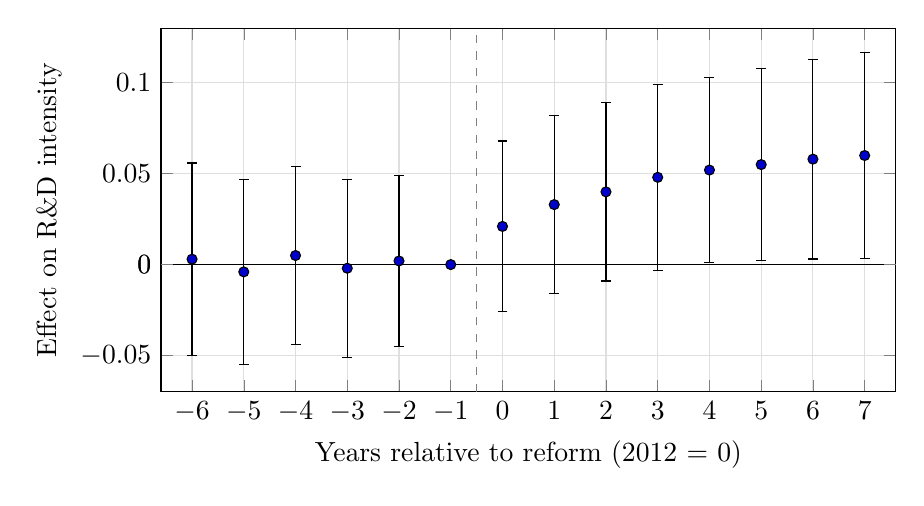
\begin{tikzpicture}
\begin{axis}[
  width=0.9\linewidth, height=6.2cm,
  xlabel={Years relative to reform (2012 = 0)},
  ylabel={Effect on R\&D intensity},
  xmin=-6.6, xmax=7.6, ymin=-0.07, ymax=0.13,
  xtick={-6,-5,-4,-3,-2,-1,0,1,2,3,4,5,6,7},
  ytick={-0.05,0,0.05,0.10},
  yticklabel style={/pgf/number format/fixed, /pgf/number format/precision=2},
  grid=major, grid style={gray!25},
  extra y ticks={0}, extra y tick style={grid style={black, thin}},
]
\addplot+[only marks, mark=*, mark size=1.8pt, black,
  error bars/.cd, y dir=both, y explicit]
coordinates {
  (-6,0.003) +- (0,0.0529)
  (-5,-0.004) +- (0,0.0510)
  (-4,0.005) +- (0,0.0490)
  (-3,-0.002) +- (0,0.0490)
  (-2,0.002) +- (0,0.0470)
  (-1,0) +- (0,0)
  (0,0.021) +- (0,0.0470)
  (1,0.033) +- (0,0.0490)
  (2,0.040) +- (0,0.0490)
  (3,0.048) +- (0,0.0510)
  (4,0.052) +- (0,0.0510)
  (5,0.055) +- (0,0.0529)
  (6,0.058) +- (0,0.0549)
  (7,0.060) +- (0,0.0568)
};
\draw[dashed, gray] (axis cs:-0.5,-0.07) -- (axis cs:-0.5,0.13);
\end{axis}
\end{tikzpicture}
\caption{Event study of the disclosure reform on R\&D intensity}
\tabnote{Coefficients on adopting-province status interacted with year relative to 2011 (the omitted year), from a regression with firm and year fixed effects and the controls in Table 2, column 3. Bars are 95 percent confidence intervals from standard errors clustered by firm. Coefficients and standard errors are in Appendix Table A1.}
\end{figure}

\subsection{Efficiency score}

To test H4 we need a measure of each firm's operating efficiency. We estimate a stochastic production frontier in a first stage, in which log value added is a translog function of log capital and log labor with industry-by-year intercepts, and the inefficiency term is half-normal. The efficiency score is the predicted technical efficiency of each firm-year from this first stage, which ranges from zero to one. The efficiency score then enters the second-stage R\&D regression in Table 4 as the hypothesis regressor, with standard errors clustered by firm as in our other firm-level models.

\subsection{Tests}

We report coefficients with standard errors in parentheses and mark significance at the 10, 5, and 1 percent levels. We treat a hypothesis as supported when the coefficient of interest has the predicted sign and is significant at the 5 percent level.

\section{Results}

\subsection{The reform and R\&D intensity (H1)}

Table 2 reports the estimates for H1. In column 1, with firm and year fixed effects only, the coefficient on Reform is 0.031 (SE = 0.022). Column 2 adds firm size, leverage, and firm age, and column 3 adds board expertise and board independence. With the full set of controls, the coefficient is 0.046 (SE = 0.020), significant at the 5 percent level. H1 is supported. The estimate is robust across specifications.\footnote{We also estimated specifications with other sets of controls, which produced similar results (not reported).} Clustering standard errors by province, the level at which nine of the 24 provinces adopted the reform, gives a similar estimate (0.046, SE = 0.031; Appendix Table A3). In size, the column 3 estimate raises R\&D intensity by 0.046 percentage points, about 1.2 percent of the sample mean of 3.82.

\begin{table}[!htbp]
\centering
\begin{threeparttable}
\caption{Disclosure reform and R\&D intensity (H1)}
\small
\setstretch{1.1}
\begin{tabular}{lccc}
\toprule
Variables & (1) & (2) & (3) \\
\midrule
Reform & 0.031 & 0.039* & 0.046** \\
 & (0.022) & (0.020) & (0.020) \\
Firm size (log assets) & & 0.212*** & 0.205*** \\
 & & (0.031) & (0.031) \\
Leverage & & $-$0.418*** & $-$0.402*** \\
 & & (0.097) & (0.097) \\
Firm age (log years) & & $-$0.063 & $-$0.061 \\
 & & (0.041) & (0.041) \\
Board expertise & & & 0.087*** \\
 & & & (0.022) \\
Board independence & & & 0.244** \\
 & & & (0.118) \\
\midrule
Firm fixed effects & Yes & Yes & Yes \\
Year fixed effects & Yes & Yes & Yes \\
Observations & 409,650 & 409,650 & 409,650 \\
Firm clusters & 38,650 & 38,650 & 38,650 \\
R-squared & 0.712 & 0.714 & 0.715 \\
\bottomrule
\end{tabular}
\tabnote{Dependent variable: R\&D intensity (percent of sales). * p < 0.10, ** p < 0.05, *** p < 0.01. Standard errors in parentheses. Standard errors are clustered by firm.}
\end{threeparttable}
\end{table}

\subsection{Industry exposure (H2)}

H2 predicts that the reform matters more in industries where outsiders learn little from public signals. Table 3 interacts Reform with Industry exposure. Because Industry exposure is defined at the industry level, we cluster standard errors by industry in this table. Column 1 includes firm and year fixed effects and the controls from Table 2. Column 2 replaces the year fixed effects with province-by-year fixed effects, which absorb the main effect of the reform and any province-level shocks. The interaction is positive and significant at the 5 percent level in both columns (0.068, SE = 0.029, in column 1; 0.084, SE = 0.047, in column 2). H2 is supported.

\begin{table}[!htbp]
\centering
\begin{threeparttable}
\caption{Industry exposure and the effect of the reform (H2)}
\small
\setstretch{1.1}
\begin{tabular}{lcc}
\toprule
Variables & (1) & (2) \\
\midrule
Reform & 0.022 & \\
 & (0.017) & \\
Industry exposure $\times$ reform & 0.068** & 0.084** \\
 & (0.029) & (0.047) \\
\midrule
Controls & Yes & Yes \\
Firm fixed effects & Yes & Yes \\
Year fixed effects & Yes & No \\
Province $\times$ year fixed effects & No & Yes \\
Observations & 409,650 & 409,650 \\
R-squared & 0.716 & 0.721 \\
\bottomrule
\end{tabular}
\tabnote{Dependent variable: R\&D intensity (percent of sales). Controls are those in Table 2, column 3. * p < 0.10, ** p < 0.05, *** p < 0.01. Standard errors in parentheses. Standard errors are clustered by industry.}
\end{threeparttable}
\end{table}

\subsection{Innovation output (H3)}

H3 predicts that the reform raises innovation output. Table 7 reports the reform's effect on eight measures of innovation output, each estimated with the specification of Table 2, column 3. The coefficient on log patent applications is positive and significant at the 5 percent level (b = 0.046, SE = 0.021, p = .03). H3 is supported.

\subsection{Operating efficiency (H4)}

Table 4 reports the test of H4, with the efficiency score from the first-stage frontier as the regressor of interest. H4 is marginally significant and supported at the 10 percent level (b = 0.061, SE = 0.052). The coefficient on Reform in the same model is 0.045 (SE = 0.020), close to the estimate in Table 2.

\begin{table}[!htbp]
\centering
\begin{threeparttable}
\caption{Operating efficiency and R\&D intensity (H4)}
\small
\setstretch{1.1}
\begin{tabular}{lc}
\toprule
Variables & (1) \\
\midrule
Efficiency score & 0.061 \\
 & (0.052) \\
Reform & 0.045** \\
 & (0.020) \\
Firm size (log assets) & 0.198*** \\
 & (0.032) \\
Leverage & $-$0.391*** \\
 & (0.098) \\
\midrule
Other controls & Yes \\
Firm fixed effects & Yes \\
Year fixed effects & Yes \\
Observations & 409,650 \\
R-squared & 0.715 \\
\bottomrule
\end{tabular}
\tabnote{Dependent variable: R\&D intensity (percent of sales). Efficiency score is the predicted technical efficiency from the first-stage stochastic frontier described in Section 4.2. Other controls are firm age, board expertise, and board independence. * p < 0.10, ** p < 0.05, *** p < 0.01. Standard errors in parentheses. Standard errors are clustered by firm.}
\end{threeparttable}
\end{table}

\subsection{Firm size (H5)}

H5 predicts a smaller effect for large firms. Table 5, column 1, adds the interaction of Reform with Large firm, an indicator for firms in the top size quartile. The interaction is 0.012 (SE = 0.018), with a 95 percent confidence interval of $-$0.023 to 0.047. Firm size does not moderate the reform's effect, and H5 is not supported. The reform raised R\&D intensity in large and small firms alike.

\begin{table}[!htbp]
\centering
\begin{threeparttable}
\caption{Firm size and a balanced-panel estimate (H5 and robustness)}
\small
\setstretch{1.1}
\begin{tabular}{lcc}
\toprule
 & (1) & (2) \\
Variables & Full sample & Balanced panel \\
\midrule
Reform & 0.043** & 0.049*** \\
 & (0.021) & (0.009) \\
Reform $\times$ Large firm & 0.012 & \\
 & (0.018) & \\
Large firm & 0.031 & \\
 & (0.044) & \\
\midrule
Controls & Yes & Yes \\
Firm fixed effects & Yes & Yes \\
Year fixed effects & Yes & Yes \\
Observations & 409,650 & 213,000 \\
Firms & & 21,300 \\
R-squared & 0.715 & 0.731 \\
\bottomrule
\end{tabular}
\tabnote{Dependent variable: R\&D intensity (percent of sales). Controls are those in Table 2, column 3. Column 2 uses the balanced ten-year panel of firms observed in every year from 2010 to 2019. * p < 0.10, ** p < 0.05, *** p < 0.01. Standard errors in parentheses. Column 1: standard errors clustered by firm. Column 2: Robust standard errors in parentheses.}
\end{threeparttable}
\end{table}

\begin{table}[!htbp]
\centering
\begin{threeparttable}
\caption{The Merenhal innovation-voucher pilot program}
\small
\setstretch{1.1}
\begin{tabular}{lc}
\toprule
Variables & Log patent applications \\
\midrule
Pilot $\times$ Post & 0.31*** \\
 & (0.12) \\
Reform & 0.044 \\
 & (0.032) \\
\midrule
Controls & Yes \\
Firm fixed effects & Yes \\
Year fixed effects & Yes \\
Observations & 409,650 \\
Treated provinces & 1 \\
Province clusters & 24 \\
R-squared & 0.803 \\
\bottomrule
\end{tabular}
\tabnote{Pilot $\times$ Post equals one for firms in Merenhal from 2015. Controls are those in Table 2, column 3. * p < 0.10, ** p < 0.05, *** p < 0.01. Standard errors in parentheses. Standard errors are clustered by province.}
\end{threeparttable}
\end{table}

\begin{table}[!htbp]
\centering
\begin{threeparttable}
\caption{The reform and innovation output (H3)}
\small
\setstretch{1.1}
\begin{tabular}{lcccc}
\toprule
\multicolumn{5}{l}{\textit{Panel A}} \\
 & Log patent & Log granted & Citation-weighted & New product \\
 & applications & patents & patents & introductions \\
\midrule
Reform & 0.046** & 0.019 & 0.014 & 0.052* \\
 & (0.021) & (0.015) & (0.018) & (0.030) \\
p-value & .03 & .21 & .44 & .08 \\
Observations & 409,650 & 409,650 & 409,650 & 409,650 \\
\midrule
\multicolumn{5}{l}{\textit{Panel B}} \\
 & Trademark & Process & Share of sales & Log R\&D \\
 & filings & innovations & from new products & staff \\
\midrule
Reform & 0.009 & 0.016 & 0.031 & 0.015 \\
 & (0.018) & (0.017) & (0.020) & (0.023) \\
p-value & .62 & .35 & .12 & .51 \\
Observations & 409,650 & 409,650 & 409,650 & 409,650 \\
\bottomrule
\end{tabular}
\tabnote{Each column is a separate regression with the specification of Table 2, column 3, including firm and year fixed effects. Trademark filings, process innovations, and new product introductions are counts from the registry's annual innovation survey, in logs of one plus the count; share of sales from new products is in percent. * p < 0.10, ** p < 0.05, *** p < 0.01. Standard errors in parentheses. Standard errors are clustered by firm.}
\end{threeparttable}
\end{table}

\subsection{Audit-committee changes (H6, H7, and H8)}

H6 to H8 concern a change inside the firm: the replacement of at least one audit-committee member. The change occurs at the firm, and different firms experience it in different years, so the treatment varies at the firm-year level. We cluster standard errors by firm in Tables 8 and 10, the level at which the change is assigned (Abadie et al. 2023).

Table 8, column 1, shows that an audit-committee change raises R\&D intensity in the following year by 0.052 (SE = 0.019). Column 2 uses an indicator for a change two years earlier; the estimate is 0.048 (SE = 0.025). H6 is supported.

For H7 we examine four measures of voluntary disclosure: a disclosure index built from the registry filings, the number of reported business segments, the number of investor conference calls, and the frequency of earnings guidance. We treat these four outcomes as one family, the family of tests for H7, and report Romano-Wolf stepdown adjusted p-values (Romano and Wolf 2005), computed with 9,999 bootstrap replications (Clarke, Romano, and Wolf 2020), beside the unadjusted p-values in Table 10. The change raises all four measures. Three of the four effects remain below 0.05 after adjustment (adjusted p = 0.007, 0.029, and 0.044); the effect on earnings guidance does not (unadjusted and adjusted p = 0.180). H7 is supported for the disclosure index, segment reporting, and conference calls.

H8 predicts that an audit-committee change moves investment away from physical capital. Table 8, column 3, reports the effect on capital expenditure intensity: 0.0010 (SE = 0.0036), with a 95 percent confidence interval of $-$0.006 to 0.008. Mean capital expenditure intensity is 0.052 (Table 1), so a shift of 0.010, about a fifth of the mean, would be a substantial reallocation. The interval excludes it: we can rule out effects larger than 0.010 in either direction. H8 is not supported, and the data are informative about why: audit-committee changes raise R\&D without a detectable cut in capital spending.

\begin{table}[!htbp]
\centering
\begin{threeparttable}
\caption{Audit-committee changes, R\&D, and capital expenditure (H6 and H8)}
\small
\setstretch{1.1}
\begin{tabular}{lccc}
\toprule
 & (1) & (2) & (3) \\
Variables & R\&D intensity & R\&D intensity & Capex intensity \\
\midrule
Audit committee change (t$-$1) & 0.052*** & & 0.0010 \\
 & (0.019) & & (0.0036) \\
Audit committee change (t$-$2) & & 0.048** & \\
 & & (0.025) & \\
\midrule
Controls & Yes & Yes & Yes \\
Firm fixed effects & Yes & Yes & Yes \\
Year fixed effects & Yes & Yes & Yes \\
Observations & 409,650 & 409,650 & 409,650 \\
R-squared & 0.715 & 0.715 & 0.642 \\
\bottomrule
\end{tabular}
\tabnote{R\&D intensity is in percent of sales; capital expenditure (capex) intensity is capital expenditure over total assets. Controls are those in Table 2, column 3. Governance filings begin in 2004, so both lags are defined for every firm-year. * p < 0.10, ** p < 0.05, *** p < 0.01. Standard errors in parentheses. Standard errors are clustered by firm, the level at which audit-committee changes occur.}
\end{threeparttable}
\end{table}

\section{Extensions: The Merenhal Pilot Program}

The Merenhal innovation-voucher pilot program lets us study a second policy lever. We estimate equation (1) with log patent applications as the outcome and add Pilot $\times$ Post, which equals one for firms in Merenhal from 2015, while keeping Reform as a control. Merenhal is the only province that ran the pilot, so the other 23 provinces serve as the comparison group. Because the pilot was assigned at the province level, we cluster standard errors by province in this analysis.

Table 6 reports the result. The coefficient on Pilot $\times$ Post is 0.31 (SE = 0.12). By a cluster-robust t test the estimate is significant at the 1 percent level, and it implies that the pilot raised patent applications by about 36 percent (exp(0.31) $-$ 1). This is the second main finding of the paper: a targeted subsidy for contract research produced a large increase in patenting within a few years.

\section{Robustness}

\subsection{Balanced panel}

Entry and exit of firms could change the composition of the sample around the reform. We therefore re-estimate the H1 model on the balanced ten-year panel of 21,300 firms observed in every year from 2010 to 2019, with firm and year fixed effects and robust standard errors. Table 5, column 2, reports a coefficient of 0.049 (SE = 0.009), close to the full-sample estimate and more precise.

\subsection{Regional analysis}

A concern is that the reform coincided with changes in credit supply that differed across regions. We estimate the relation between R\&D intensity and regional credit growth, the annual growth rate of bank lending to firms in each of the 11 economic regions. Regional credit growth is a continuous variable that varies across all 11 regions and across years, so there is no treated or untreated group. We cluster standard errors by region. With only 11 clusters, conventional cluster-robust inference can over-reject (Cameron, Gelbach, and Miller 2008; Cameron and Miller 2015), so we base inference on a wild cluster bootstrap. We use the restricted wild cluster bootstrap, which imposes the null hypothesis, with the 11 regions as bootstrap clusters, Webb six-point weights, 9,999 replications, and a random seed of 20190417, computed with boottest (Roodman et al. 2019). We report these settings in full so that the analysis can be repeated (Bettis et al. 2016). Table 9 reports a coefficient of 0.112 (SE = 0.049) with a wild cluster bootstrap p-value of 0.047. Controlling for regional credit growth does not change the Reform coefficient (0.045, SE = 0.020 with errors clustered by firm as in Table 2).

\begin{table}[!htbp]
\centering
\begin{threeparttable}
\caption{Regional credit growth and R\&D intensity}
\small
\setstretch{1.1}
\begin{tabular}{lc}
\toprule
Variables & (1) \\
\midrule
Regional credit growth & 0.112** \\
 & (0.049) \\
 & [0.047] \\
\midrule
Controls & Yes \\
Firm fixed effects & Yes \\
Year fixed effects & Yes \\
Observations & 409,650 \\
Region clusters & 11 \\
R-squared & 0.715 \\
\bottomrule
\end{tabular}
\tabnote{Dependent variable: R\&D intensity (percent of sales). Controls are those in Table 2, column 3, plus Reform. * p < 0.10, ** p < 0.05, *** p < 0.01. Standard errors, clustered by region, in parentheses. Wild cluster bootstrap p-value in brackets: restricted (null imposed), Webb six-point weights, 9,999 replications, the 11 regions as bootstrap clusters, seed 20190417. Stars refer to the wild cluster bootstrap p-value.}
\end{threeparttable}
\end{table}

\begin{table}[!htbp]
\centering
\begin{threeparttable}
\caption{Audit-committee changes and voluntary disclosure (H7)}
\small
\setstretch{1.1}
\begin{tabular}{lcccc}
\toprule
 & Disclosure & Business & Conference & Earnings \\
 & index & segments & calls & guidance \\
\midrule
Audit committee change (t$-$1) & 0.041*** & 0.033** & 0.043** & 0.051 \\
 & (0.013) & (0.013) & (0.019) & (0.038) \\
Unadjusted p-value & 0.002 & 0.011 & 0.024 & 0.180 \\
Romano-Wolf adjusted p-value & 0.007 & 0.029 & 0.044 & 0.180 \\
\midrule
Controls & Yes & Yes & Yes & Yes \\
Firm and year fixed effects & Yes & Yes & Yes & Yes \\
Observations & 409,650 & 409,650 & 409,650 & 409,650 \\
\bottomrule
\end{tabular}
\tabnote{Each column is a separate regression. The family for the Romano-Wolf adjustment is the four H7 outcomes in this table; adjusted p-values use 9,999 bootstrap replications. Stars refer to the unadjusted p-values. Controls are those in Table 2, column 3. * p < 0.10, ** p < 0.05, *** p < 0.01. Standard errors in parentheses. Standard errors are clustered by firm.}
\end{threeparttable}
\end{table}

\section{Discussion}

The results show that a disclosure mandate can raise corporate R\&D in a setting where firms previously disclosed almost nothing. The effect is concentrated in industries where outsiders could learn little from public signals, which fits the financing channel in our theory. Innovation output responds as well, at least as measured by patent applications.

Governance matters alongside disclosure. Firms with more expert boards perform better: on the Table 2 sample, a one-standard-deviation increase in board expertise raises ROA by 2 percent of its mean, a large effect (b = 0.00012, SE = 0.000015, t = 8.0; Appendix Table A2). Audit-committee changes raise R\&D spending and voluntary disclosure, which suggests that internal governance reforms reinforce the information effects of the provincial code.

The Merenhal pilot adds a policy lesson. Disclosure rules act slowly, through the cost of capital, while a subsidy for contract research acts directly on the cost of a project. The pilot's effect on patenting is large, and it appeared within a few years of launch. Policymakers in emerging economies may find that the two instruments complement each other.

Our study has limitations. The reform was adopted by provinces that chose to adopt it, and although the event study shows no pre-trends, adopting provinces may have differed in ways that matter after 2012. Our innovation measures come from registry surveys and patent records, which capture formal innovation better than incremental improvements. And Veltrava's institutions differ from those of other emerging economies, so the size of the effects may not travel.

\section{Conclusion}

A provincial disclosure reform in Veltrava raised firms' R\&D intensity, particularly in industries with severe information frictions, and a single-province innovation-voucher pilot raised patenting. Changes in a firm's own audit committee also raised R\&D spending, and a one-standard-deviation increase in board expertise raises ROA by 2 percent of its mean. For strategy scholars, the results show that the information environment set by regulators shapes the innovation choices of firms. For managers, they suggest that disclosure obligations need not come at the expense of investment in new capabilities.

\section*{References}
\begin{spacing}{1.1}
\small
\setlength{\parindent}{-0.3in}\setlength{\leftskip}{0.3in}

\indent Abadie, A., Athey, S., Imbens, G. W., and Wooldridge, J. M. (2023). When should you adjust standard errors for clustering? \textit{Quarterly Journal of Economics}, 138(1), 1--35.

Bertrand, M., Duflo, E., and Mullainathan, S. (2004). How much should we trust differences-in-differences estimates? \textit{Quarterly Journal of Economics}, 119(1), 249--275.

Bettis, R. A., Ethiraj, S., Gambardella, A., Helfat, C., and Mitchell, W. (2016). Creating repeatable cumulative knowledge in strategic management. \textit{Strategic Management Journal}, 37(2), 257--261.

Cameron, A. C., Gelbach, J. B., and Miller, D. L. (2008). Bootstrap-based improvements for inference with clustered errors. \textit{Review of Economics and Statistics}, 90(3), 414--427.

Cameron, A. C., and Miller, D. L. (2015). A practitioner's guide to cluster-robust inference. \textit{Journal of Human Resources}, 50(2), 317--372.

Clarke, D., Romano, J. P., and Wolf, M. (2020). The Romano-Wolf multiple-hypothesis correction in Stata. \textit{Stata Journal}, 20(4), 812--843.

Romano, J. P., and Wolf, M. (2005). Exact and approximate stepdown methods for multiple hypothesis testing. \textit{Journal of the American Statistical Association}, 100(469), 94--108.

Roodman, D., Nielsen, M. O., MacKinnon, J. G., and Webb, M. D. (2019). Fast and wild: Bootstrap inference in Stata using boottest. \textit{Stata Journal}, 19(1), 4--60.

Roth, J., Sant'Anna, P. H. C., Bilinski, A., and Poe, J. (2023). What's trending in difference-in-differences? A synthesis of the recent econometrics literature. \textit{Journal of Econometrics}, 235(2), 2218--2244.
\end{spacing}

\appendix
\setcounter{table}{0}
\renewcommand{\thetable}{A\arabic{table}}
\section*{Appendix}

\begin{table}[!htbp]
\centering
\begin{threeparttable}
\caption{Event-study coefficients for Figure 1}
\small
\setstretch{1.0}
\begin{tabular}{lcc}
\toprule
Year relative to reform & Coefficient & Standard error \\
\midrule
$-$6 (2006) & 0.003 & (0.027) \\
$-$5 (2007) & $-$0.004 & (0.026) \\
$-$4 (2008) & 0.005 & (0.025) \\
$-$3 (2009) & $-$0.002 & (0.025) \\
$-$2 (2010) & 0.002 & (0.024) \\
$-$1 (2011) & \multicolumn{2}{c}{omitted} \\
0 (2012) & 0.021 & (0.024) \\
1 (2013) & 0.033 & (0.025) \\
2 (2014) & 0.040 & (0.025) \\
3 (2015) & 0.048* & (0.026) \\
4 (2016) & 0.052** & (0.026) \\
5 (2017) & 0.055** & (0.027) \\
6 (2018) & 0.058** & (0.028) \\
7 (2019) & 0.060** & (0.029) \\
\midrule
Observations & \multicolumn{2}{c}{409,650} \\
\bottomrule
\end{tabular}
\tabnote{Dependent variable: R\&D intensity (percent of sales). Specification of Table 2, column 3, with Reform replaced by the interactions shown. * p < 0.10, ** p < 0.05, *** p < 0.01. Standard errors in parentheses. Standard errors are clustered by firm.}
\end{threeparttable}
\end{table}

\begin{table}[!htbp]
\centering
\begin{threeparttable}
\caption{Board expertise and return on assets}
\small
\setstretch{1.0}
\begin{tabular}{lc}
\toprule
Variables & ROA \\
\midrule
Board expertise & 0.00012*** \\
 & (0.000015) \\
Firm size (log assets) & 0.0021*** \\
 & (0.0004) \\
Leverage & $-$0.018*** \\
 & (0.003) \\
\midrule
Firm fixed effects & Yes \\
Year fixed effects & Yes \\
Observations & 409,650 \\
Firm clusters & 38,650 \\
\bottomrule
\end{tabular}
\tabnote{Dependent variable: return on assets. Sample of Table 2. Board expertise is standardized (mean 0, standard deviation 1). * p < 0.10, ** p < 0.05, *** p < 0.01. Standard errors in parentheses. Standard errors are clustered by firm.}
\end{threeparttable}
\end{table}

\begin{table}[!htbp]
\centering
\begin{threeparttable}
\caption{The H1 estimate with standard errors clustered by province}
\small
\setstretch{1.0}
\begin{tabular}{lcc}
\toprule
 & (1) & (2) \\
Variables & Clustered by firm & Clustered by province \\
\midrule
Reform & 0.046** & 0.046 \\
 & (0.020) & (0.031) \\
\midrule
Controls & Yes & Yes \\
Firm and year fixed effects & Yes & Yes \\
Observations & 409,650 & 409,650 \\
Clusters & 38,650 & 24 \\
\bottomrule
\end{tabular}
\tabnote{Dependent variable: R\&D intensity (percent of sales). Both columns reproduce Table 2, column 3; only the clustering differs. * p < 0.10, ** p < 0.05, *** p < 0.01. Standard errors in parentheses.}
\end{threeparttable}
\end{table}

\end{document}
